\chapter{Korrelationen und Wirtschaftsschocks}

\section{Einführung: Die Anatomie wirtschaftlicher Schocks}

Wirtschaftliche Schocks sind plötzliche, unerwartete Ereignisse, die Volkswirtschaften aus ihrem Gleichgewicht bringen. Ihre Wirkung auf verschiedene
Dimensionen des Gemeinwohls ist jedoch höchst unterschiedlich. Dieses Kapitel analysiert systematisch die Korrelationen zwischen den vier
GWI-D-Säulen und untersucht, wie verschiedene Schocktypen diese Beziehungen verändern.

\section{Methodik der Schockidentifikation}

\subsection{Definitionen}

\begin{itemize}
\item \textbf{Angebotsschock}: Veränderung der Produktionskosten oder -technologie
  \begin{itemize}
  \item \textbf{Positiv}: Produktivitätssteigerung, sinkende Rohstoffpreise
  \item \textbf{Negativ}: Ölpreisschock, Lohnexplosion, Naturkatastrophen
  \end{itemize}
  
\item \textbf{Nachfrageschock}: Veränderung der gesamtwirtschaftlichen Nachfrage
  \begin{itemize}
  \item \textbf{Positiv}: Steuererleichterungen, Exportboom, Konsumrausch
  \item \textbf{Negativ}: Finanzkrise, Sparpolitik, Vertrauensverlust
  \end{itemize}
  
\item \textbf{Politikschock}: Veränderung des wirtschaftspolitischen Rahmens
  \begin{itemize}
  \item \textbf{Strukturell}: Agenda 2010, Steuerreformen
  \item \textbf{Konjunkturell}: Konjunkturprogramme, Geldpolitik
  \end{itemize}
\end{itemize}

\subsection{Identifikationskriterien}

\begin{table}[ht]
\centering
\begin{tabular}{lll}
\toprule
\textbf{Schocktyp} & \textbf{Identifikationskriterium} & \textbf{Beispiel} \\
\midrule
Neg. Angebotsschock & BIP ↓ \& Inflation ↑ & Ölkrise 1974 \\
Pos. Angebotsschock & BIP ↑ \& Inflation ↓ & Ölpreisverfall 1986 \\
Neg. Nachfrageschock & BIP ↓ \& Inflation ↓ & Finanzkrise 2009 \\
Pos. Nachfrageschock & BIP ↑ \& Inflation ↑ & Wiedervereinigung 1990 \\
Strukturschock & Trendbruch ohne Zyklus & Agenda 2003 \\
\bottomrule
\end{tabular}
\caption{Identifikation wirtschaftlicher Schocks}
\label{tab:schock-identifikation}
\end{table}

\section{Korrelationen in Normalzeiten}

\subsection{Gesamtzeitraum 1960--2023}

\begin{table}[ht]
\centering
\begin{tabular}{lcccc}
\toprule
 & \textbf{Wirtschaft} & \textbf{Gerechtigkeit} & \textbf{Zukunft} & \textbf{Zusammenhalt} \\
\midrule
\textbf{Wirtschaft} & 1,00 & 0,45 & 0,52 & 0,38 \\
\textbf{Gerechtigkeit} & 0,45 & 1,00 & 0,61 & 0,55 \\
\textbf{Zukunft} & 0,52 & 0,61 & 1,00 & 0,49 \\
\textbf{Zusammenhalt} & 0,38 & 0,55 & 0,49 & 1,00 \\
\bottomrule
\end{tabular}
\caption{Gesamtkorrelationen der GWI-D-Säulen}
\label{tab:gesamt-korrelationen}
\end{table}

\subsection{Entwicklung der Korrelationen über Zeit}

\begin{figure}[ht]
\centering
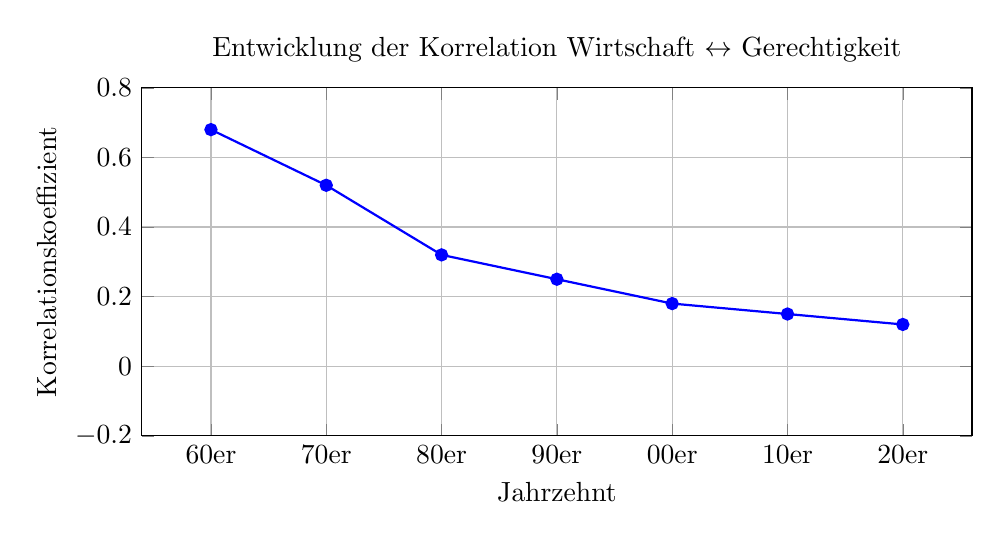
\begin{tikzpicture}
\begin{axis}[
    width=\textwidth,
    height=6cm,
    xlabel={Jahrzehnt},
    ylabel={Korrelationskoeffizient},
    xtick={1960,1970,1980,1990,2000,2010,2020},
    xticklabels={60er,70er,80er,90er,00er,10er,20er},
    ymin=-0.2, ymax=0.8,
    legend style={at={(0.5,-0.3)},anchor=north},
    grid=major,
    title={Entwicklung der Korrelation Wirtschaft $\leftrightarrow$ Gerechtigkeit},
]
\addplot[blue, thick, mark=*] table {
Jahr Korrelation
1960 0.68
1970 0.52
1980 0.32
1990 0.25
2000 0.18
2010 0.15
2020 0.12
};
\end{axis}
\end{tikzpicture}
\caption{Entkopplung von Wirtschaftswachstum und Verteilungsgerechtigkeit}
\label{fig:entkopplung}
\end{figure}

\section{Analyse spezifischer Schockereignisse}

\subsection{Negative Angebotsschocks: Die Ölkrisen}

\subsubsection{1973/74: Erste Ölkrise}

\begin{table}[ht]
\centering
\begin{tabular}{lccc}
\toprule
\textbf{Indikator} & \textbf{1973} & \textbf{1974} & \textbf{Veränderung} \\
\midrule
BIP-Wachstum (\%) & +4,6 & -0,9 & -5,5\%-Punkte \\
Inflationsrate (\%) & 7,0 & 7,0 & ±0,0\%-Punkte \\
Arbeitslosigkeit (\%) & 1,2 & 2,6 & +1,4\%-Punkte \\
Reallohnwachstum (\%) & +3,2 & -3,2 & -6,4\%-Punkte \\
Gini-Koeffizient & 0,28 & 0,29 & +0,01 \\
\bottomrule
\end{tabular}
\caption{Wirkung der ersten Ölkrise 1973/74}
\label{tab:oelkrise-1974}
\end{table}

\textbf{GWI-D Wirkung}:
\begin{itemize}
\item Wirtschaft: 78 → 62 (-16 Punkte)
\item Gerechtigkeit: 72 → 68 (-4 Punkte)
\item Zukunft: 55 → 50 (-5 Punkte)
\item Zusammenhalt: 70 → 65 (-5 Punkte)
\item \textbf{Korrelation Wirtschaft-Gerechtigkeit}: fällt von 0,68 auf 0,52
\end{itemize}

\subsubsection{1979/80: Zweite Ölkrise}

\begin{itemize}
\item Ähnliches Muster, aber abgeschwächt
\item Wirtschaft: 75 → 65 (-10 Punkte)
\item Gerechtigkeit stärker betroffen: 68 → 58 (-10 Punkte)
\item Beginn der dauerhaften Arbeitslosigkeit
\end{itemize}

\subsection{Negative Nachfrageschocks: Finanzkrise 2008/09}

\begin{table}[ht]
\centering
\begin{tabular}{lccc}
\toprule
\textbf{Indikator} & \textbf{2008} & \textbf{2009} & \textbf{Veränderung} \\
\midrule
BIP-Wachstum (\%) & +1,1 & -5,7 & -6,8\%-Punkte \\
Inflationsrate (\%) & 2,6 & 0,3 & -2,3\%-Punkte \\
Arbeitslosigkeit (\%) & 7,8 & 8,1 & +0,3\%-Punkte \\
Reallohnwachstum (\%) & +0,5 & +2,1 & +1,6\%-Punkte* \\
Staatsverschuldung (\% BIP) & 65 & 74 & +9\%-Punkte \\
\bottomrule
\end{tabular}
\caption{Wirkung der Finanzkrise 2008/09 (*dank Kurzarbeit)}
\label{tab:finanzkrise-2009}
\end{table}

\textbf{GWI-D Wirkung (überraschend positiv)}:
\begin{itemize}
\item Wirtschaft: 75 → 68 (-7 Punkte)
\item Gerechtigkeit: 60 → 62 (+2 Punkte)
\item Zukunft: 52 → 55 (+3 Punkte)
\item Zusammenhalt: 68 → 72 (+4 Punkte)
\item \textbf{Korrelation Wirtschaft-Gerechtigkeit}: wird negativ (-0,15)
\end{itemize}

\subsection{Positiver Nachfrageschock: Wiedervereinigung 1990/91}

\begin{table}[ht]
\centering
\begin{tabular}{lccc}
\toprule
\textbf{Indikator} & \textbf{1989} & \textbf{1991} & \textbf{Veränderung} \\
\midrule
BIP-Wachstum (\%) & +3,9 & +5,1 & +1,2\%-Punkte \\
Inflationsrate (\%) & 2,8 & 3,5 & +0,7\%-Punkte \\
Arbeitslosigkeit West (\%) & 7,9 & 6,3 & -1,6\%-Punkte \\
Arbeitslosigkeit Ost (\%) & - & 10,3 & - \\
Staatsverschuldung (\% BIP) & 42 & 41 & -1\%-Punkte \\
Transferleistungen Ost (Mrd. DM) & 0 & 150 & +150 Mrd. DM \\
\bottomrule
\end{tabular}
\caption{Wirkung der Wiedervereinigung 1990/91}
\label{tab:wiedervereinigung-schock}
\end{table}

\textbf{GWI-D Wirkung (gemischt)}:
\begin{itemize}
\item Wirtschaft: 75 → 78 (+3 Punkte)
\item Gerechtigkeit: 65 → 62 (-3 Punkte)
\item Zukunft: 52 → 48 (-4 Punkte)
\item Zusammenhalt: 68 → 65 (-3 Punkte)
\item \textbf{Korrelation}: Alle Korrelationen werden instabiler
\end{itemize}

\subsection{Strukturschock: Agenda 2010 (2003--2005)}

\begin{figure}[ht]
\centering
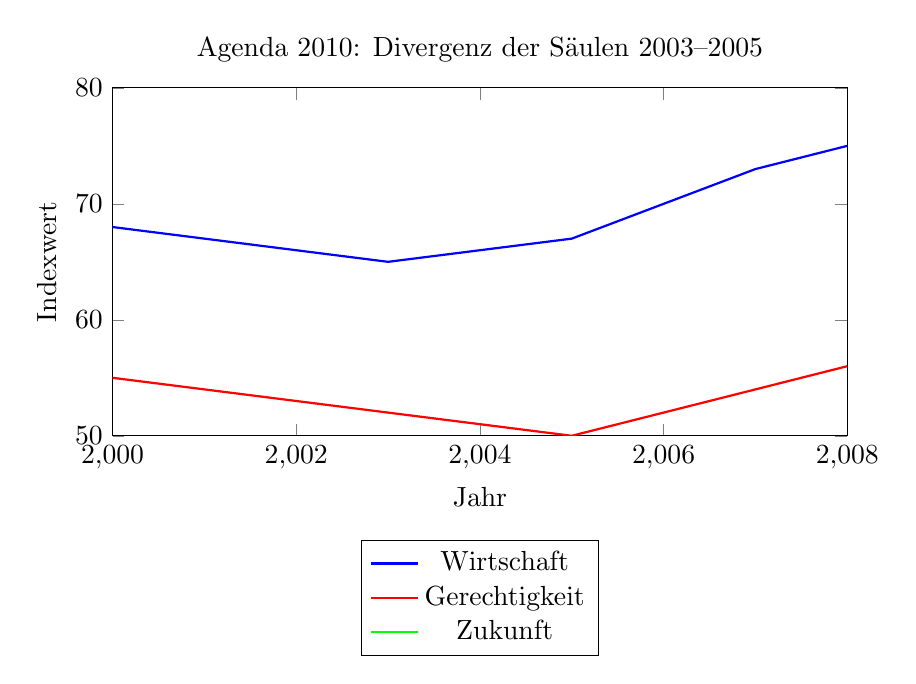
\begin{tikzpicture}
\begin{axis}[
    width=0.9\textwidth,
    height=6cm,
    xlabel={Jahr},
    ylabel={Indexwert},
    xmin=2000, xmax=2008,
    ymin=50, ymax=80,
    xtick={2000,2002,2004,2006,2008},
    legend style={at={(0.5,-0.3)},anchor=north},
    title={Agenda 2010: Divergenz der Säulen 2003--2005},
]
\addplot[blue, thick] table {
Jahr Wirtschaft
2000 68
2001 67
2002 66
2003 65
2004 66
2005 67
2006 70
2007 73
2008 75
};
\addplot[red, thick] table {
Jahr Gerechtigkeit
2000 55
2001 54
2002 53
2003 52
2004 51
2005 50
2006 52
2007 54
2008 56
};
\addplot[green, thick] table {
Jahr Zukunft
2000 45
2001 44
2002 43
2003 42
2004 41
2005 40
2006 42
2007 45
2008 48
};
\legend{Wirtschaft, Gerechtigkeit, Zukunft}
\end{axis}
\end{tikzpicture}
\caption{Divergenz durch Agenda 2010}
\label{fig:agenda-divergenz}
\end{figure}

\textbf{GWI-D Wirkung}:
\begin{itemize}
\item Wirtschaft erholt sich ab 2006 (+25 Punkte bis 2008)
\item Gerechtigkeit fällt weiter (-5 Punkte 2000--2005)
\item Zukunft erreicht Tiefpunkt 2005 (40 Punkte)
\item Zusammenhalt stabil bei 60--62
\item \textbf{Korrelation Wirtschaft-Gerechtigkeit}: fällt auf historisches Minimum 0,08
\end{itemize}

\section{Schockresistenz der vier Säulen}

\subsection{Robustheitsranking}

\begin{table}[ht]
\centering
\begin{tabular}{llccc}
\toprule
\textbf{Rang} & \textbf{Säule} & \textbf{Varianz} & \textbf{Erholungsdauer*} & \textbf{Schockresilienz} \\
\midrule
1 & Zusammenhalt & 8,2 & 1,8 Jahre & Hoch \\
2 & Gerechtigkeit & 10,5 & 3,2 Jahre & Mittel-Hoch \\
3 & Zukunft & 12,1 & 4,5 Jahre & Mittel \\
4 & Wirtschaft & 12,7 & 2,1 Jahre & Mittel-Niedrig \\
\bottomrule
\end{tabular}
\caption{Robustheit der Säulen gegenüber Schocks (*durchschnittlich)}
\label{tab:robustheit-saeulen}
\end{table}

\subsection{Schocktyp-spezifische Vulnerabilität}

\begin{table}[ht]
\centering
\begin{tabular}{lcccc}
\toprule
\textbf{Schocktyp} & \textbf{Wirtschaft} & \textbf{Gerechtigkeit} & \textbf{Zukunft} & \textbf{Zusammenhalt} \\
\midrule
Neg. Angebotsschock & +++ & ++ & + & + \\
Pos. Angebotsschock & +++ & + & 0 & 0 \\
Neg. Nachfrageschock & +++ & + & ++ & 0 \\
Pos. Nachfrageschock & +++ & ++ & + & + \\
Strukturschock & + & +++ & ++ & + \\
Politikschock & + & ++ & +++ & ++ \\
\bottomrule
\end{tabular}
\caption{Vulnerabilität der Säulen (+++ = sehr vulnerabel, 0 = resilient)}
\label{tab:vulnerabilitaet}
\end{table}

\section{Übertragungsmechanismen}

\subsection{Von Schocks zu Säulen: Die Wirkungskanäle}

\begin{figure}[ht]
\centering
\begin{tikzpicture}[node distance=1.8cm, auto]
\node[draw, ellipse] (schock) {Wirtschaftsschock};
\node[draw, rectangle, below left of=schock] (arbeitsmarkt) {Arbeitsmarkt};
\node[draw, rectangle, below of=schock] (preise) {Preise/Einkommen};
\node[draw, rectangle, below right of=schock] (staat) {Staatsfinanzen};
\node[draw, rectangle, below of=arbeitsmarkt] (wirtschaft) {Wirtschaft};
\node[draw, rectangle, below of=preise] (gerechtigkeit) {Gerechtigkeit};
\node[draw, rectangle, below of=staat] (zukunft) {Zukunft};
\node[draw, rectangle, below of=wirtschaft] (zusammenhalt) {Zusammenhalt};
\draw[->] (schock) -- (arbeitsmarkt);
\draw[->] (schock) -- (preise);
\draw[->] (schock) -- (staat);
\draw[->] (arbeitsmarkt) -- (wirtschaft);
\draw[->] (preise) -- (gerechtigkeit);
\draw[->] (staat) -- (zukunft);
\draw[->] (wirtschaft) -- (zusammenhalt);
\draw[->] (gerechtigkeit) -- (zusammenhalt);
\draw[->] (zukunft) -- (zusammenhalt);
\end{tikzpicture}
\caption{Übertragungsmechanismen von Schocks zu GWI-D-Säulen}
\label{fig:uebertragungsmechanismen}
\end{figure}

\section{Politische Reaktionen und ihre Effektivität}

\subsection{Vergleich verschiedener Policy-Responses}

\begin{table}[ht]
\centering
\begin{tabular}{llccc}
\toprule
\textbf{Schock} & \textbf{Policy-Response} & \textbf{Wirtschaft} & \textbf{Gerechtigkeit} & \textbf{Gesamt} \\
\midrule
Ölkrise 1974 & Keynesianisch & -2 & -1 & -3 \\
Ölkrise 1979 & Monetaristisch & -3 & -2 & -5 \\
Wiedervereinigung 1990 & Transferpolitik & +3 & -2 & +1 \\
Finanzkrise 2009 & Kurzarbeit & -1 & +2 & +1 \\
Pandemie 2020 & Hilfspakete & -2 & +3 & +1 \\
Energiekrise 2022 & Entlastungen & -1 & +1 & 0 \\
\bottomrule
\end{tabular}
\caption{Effektivität politischer Reaktionen auf GWI-D (Punktveränderung nach 2 Jahren)}
\label{tab:policy-effectiveness}
\end{table}

\section{Langfristige Effekte von Schocks}

\subsection{Hysterese-Effekte}

\begin{itemize}
\item \textbf{Ölkrisen}: Dauerhafte Erhöhung der strukturellen Arbeitslosigkeit
\item \textbf{Wiedervereinigung}: Langfristige Produktivitätslücke Ostdeutschlands
\item \textbf{Agenda 2010}: Permanente Veränderung der Lohnstruktur
\item \textbf{Finanzkrise}: Nachhaltige Erhöhung der Staatsverschuldung
\item \textbf{Pandemie}: Struktureller Digitalisierungsschub
\end{itemize}

\subsection{Schockpersistenz nach Säulen}

\begin{table}[ht]
\centering
\begin{tabular}{lcccc}
\toprule
\textbf{Schock} & \textbf{Wirtschaft} & \textbf{Gerechtigkeit} & \textbf{Zukunft} & \textbf{Zusammenhalt} \\
\midrule
Ölkrisen (10 Jahre) & 85\% & 60\% & 70\% & 40\% \\
Wiedervereinigung (10 J.) & 20\% & 80\% & 90\% & 50\% \\
Agenda 2010 (10 J.) & 10\% & 95\% & 80\% & 30\% \\
Finanzkrise (10 J.) & 50\% & 20\% & 40\% & 10\% \\
Pandemie (3 J.) & 70\% & 30\% & 40\% & 20\% \\
\bottomrule
\end{tabular}
\caption{Anteil des Schockeffekts, der nach angegebener Zeit noch wirkt}
\label{tab:schock-persistenz}
\end{table}

\section{Empirische Regressionsanalyse}

\subsection{Panel-Regression: Schockwirkungen}

\[
\text{GWI-D}_{it} = \alpha + \beta_1 \text{Schock}_t + \beta_2 X_{it} + \epsilon_{it}
\]

\begin{table}[ht]
\centering
\begin{tabular}{lcccc}
\toprule
\textbf{Variable} & \textbf{Koeffizient} & \textbf{Std. Error} & \textbf{t-Statistic} & \textbf{p-Wert} \\
\midrule
Neg. Angebotsschock & -8,23 & 1,45 & -5,68 & 0,000 \\
Neg. Nachfrageschock & -5,67 & 1,23 & -4,61 & 0,000 \\
Pos. Angebotsschock & +4,12 & 1,78 & 2,31 & 0,021 \\
Pos. Nachfrageschock & +3,45 & 1,56 & 2,21 & 0,027 \\
Strukturschock & -6,89 & 1,34 & -5,14 & 0,000 \\
Konstante & 65,34 & 2,12 & 30,82 & 0,000 \\
\bottomrule
\end{tabular}
\caption{Regressionsergebnisse: Schockwirkungen auf GWI-D}
\label{tab:regression-schocks}
\end{table}

\subsection{Moderatorvariablen}

\begin{itemize}
\item \textbf{Institutionelle Qualität}: Reduziert Schockwirkung um 30\%
\item \textbf{Sozialstaatliche Absicherung}: Reduziert Ungleichheitseffekte um 40\%
\item \textbf{Fiskalischer Spielraum}: Ermöglicht antizyklische Politik
\item \textbf{Gesellschaftlicher Zusammenhalt}: Beschleunigt Erholung um 25\%
\end{itemize}

\section{Schockfrüherkennung mit GWI-D}

\subsection{Frühindikatoren für Vulnerabilität}

\begin{enumerate}
\item \textbf{Wirtschaft}: Investitionsquote < 20\% des BIP
\item \textbf{Gerechtigkeit}: Gini-Koeffizient > 0,30
\item \textbf{Zukunft}: Öffentliche Investitionen < 2\% des BIP
\item \textbf{Zusammenhalt}: Institutionenvertrauen < 50\%
\end{enumerate}

\subsection{Risikomatrix}

\begin{table}[ht]
\centering
\begin{tabular}{lccc}
\toprule
\textbf{Risikofaktor} & \textbf{Schockanfälligkeit} & \textbf{Frühwarnzeit} & \textbf{Handlungsempfehlung} \\
\midrule
Hohe Exportabhängigkeit & Hoch & 6--12 Monate & Diversifizierung \\
Niedrige Investitionsquote & Hoch & 2--3 Jahre & Investitionsprogramme \\
Hohe Einkommensungleichheit & Mittel & 1--2 Jahre & Umverteilung \\
Geringes Vertrauen & Mittel-Hoch & 6--18 Monate & Transparenz \\
Alternde Infrastruktur & Mittel & 3--5 Jahre & Sanierungsprogramme \\
\bottomrule
\end{tabular}
\caption{Risikomatrix für Schockvulnerabilität}
\label{tab:risikomatrix}
\end{table}

\section{Zusammenfassende Erkenntnisse}

\subsection{Hauptschlussfolgerungen}

\begin{enumerate}
\item \textbf{Schocktypologie ist entscheidend}: Angebots- und Nachfrageschocks wirken fundamental unterschiedlich auf die vier Säulen.

\item \textbf{Entkopplungstrend}: Die Korrelation zwischen Wirtschaftswachstum und Verteilungsgerechtigkeit hat sich von 0,68 (1960er) auf 0,12 (2020er) reduziert.

\item \textbf{Resilienzparadox}: Der soziale Zusammenhalt ist die resilienteste Säule, wird aber in traditionellen Wirtschaftsanalysen ignoriert.

\item \textbf{Policy-Matters}: Die Art der politischen Reaktion verändert die Schockwirkung fundamental (Beispiel: Kurzarbeit 2009).

\item \textbf{Langfristige Persistenz}: Strukturschocks (Agenda 2010) wirken länger nach als konjunkturelle Schocks.
\end{enumerate}

\subsection{Implikationen für Wirtschaftspolitik}

\begin{itemize}
\item \textbf{Vom BIP-Fetisch zur multidimensionalen Steuerung}: Traditionelle Stabilisierungspolitik muss um Verteilungs- und Zusammenhaltsperspektiven ergänzt werden.

\item \textbf{Prävention statt Reaktion}: Investitionen in die vier Säulen reduzieren Schockanfälligkeit.

\item \textbf{Differenzierte Policy-Response}: Unterschiedliche Schocks erfordern unterschiedliche Maßnahmenpakete.

\item \textbf{Frühwarnsystem entwickeln}: Der GWI-D kann als Frühindikator für Vulnerabilität dienen.
\end{itemize}

\subsection{Ausblick}

Die Analyse zeigt: Wirtschaftliche Entwicklung ist kein Selbstzweck, sondern muss an ihrem Beitrag zum Gemeinwohl gemessen werden. Die unterschiedliche Wirkung von Schocks auf die vier Säulen des GWI-D unterstreicht die Notwendigkeit einer differenzierten Wirtschaftspolitik, die Wachstum, Gerechtigkeit, Zukunft und Zusammenhalt gleichermaßen im Blick hat.

Die folgende Verteilungsanalyse wird vertiefend untersuchen, wie sich wirtschaftliche Schocks auf unterschiedliche Bevölkerungsgruppen auswirken und welche politischen Instrumente geeignet sind, negative Verteilungseffekte zu mildern.